\documentclass{article}

\usepackage{graphicx}
\usepackage{tikz}
\usepackage{tikzsymbols}
\usetikzlibrary{calc,patterns,shapes.geometric}
\pagestyle{empty}
\usepackage[margin=0pt]{geometry}
\geometry{papersize={14in,12in}}

\def\centerarc[#1](#2)(#3:#4:#5){\draw[#1] ($(#2)+({#5*cos(#3)},{#5*sin(#3)})$) arc (#3:#4:#5);}

\begin{document}
	\begin{figure}
		\centering
		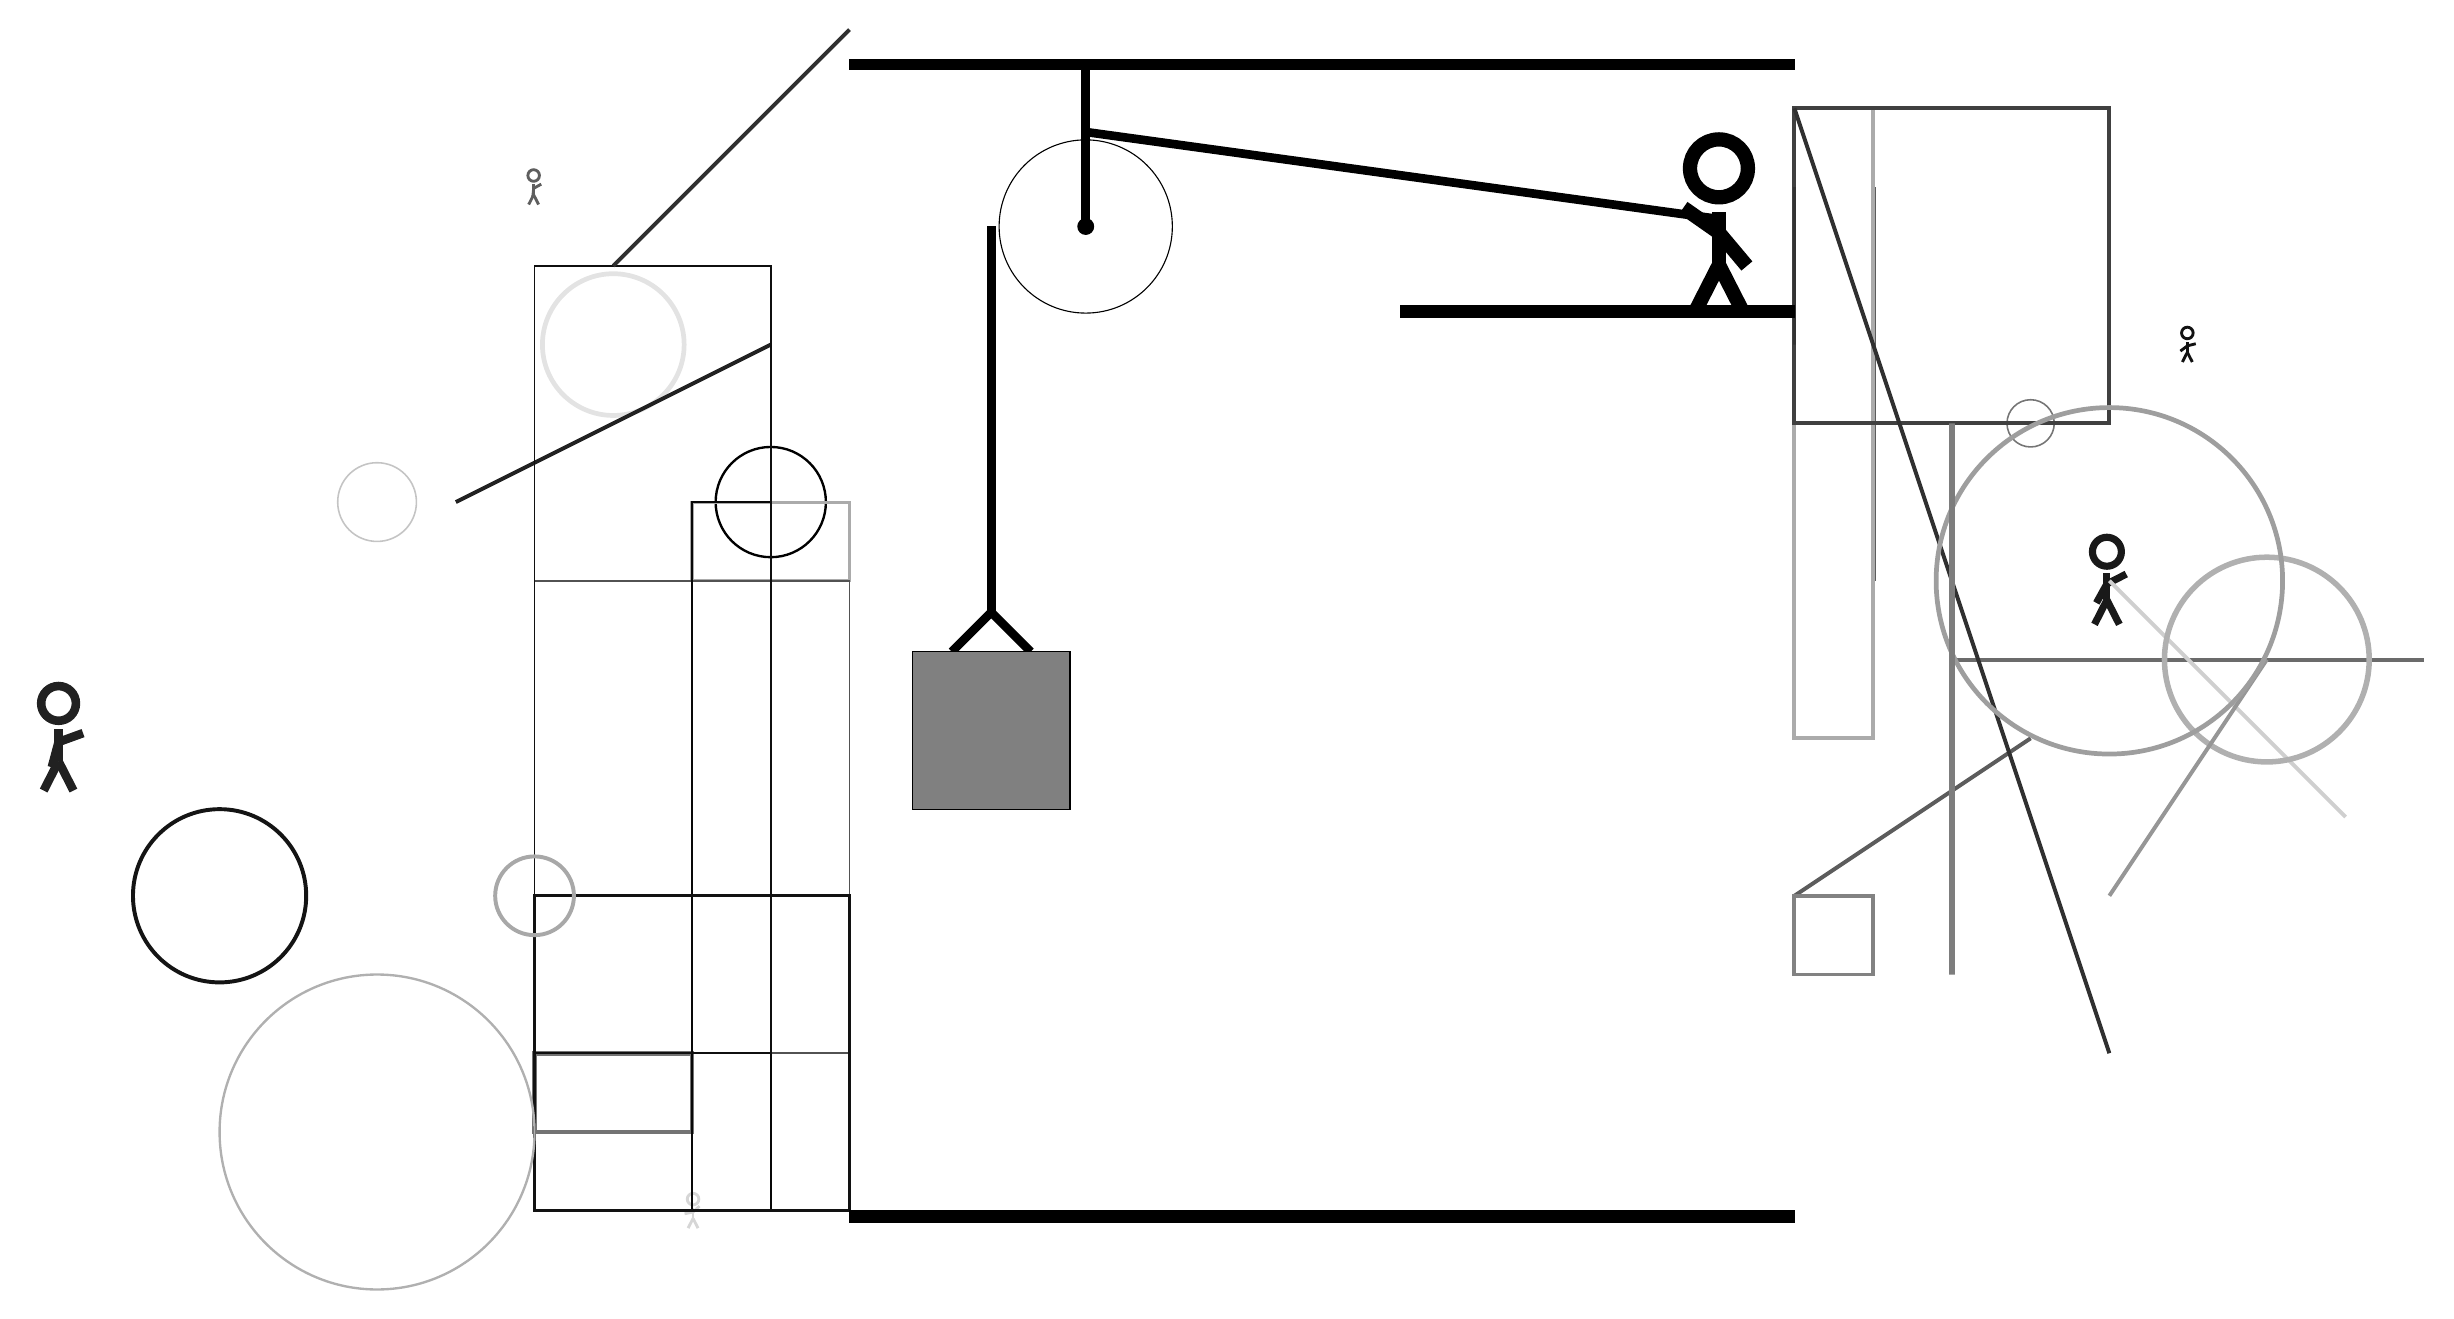
\begin{tikzpicture}
			%%%%% START %%%%%
			
			\draw[fill=black] (-2, 11.5) rectangle (10, 11.625);
			
			\node[line width=0.5mm, color=black!90] at (14, 5) {\Strichmaxerl[5][61][27]};
			
			\draw[line width=0.5mm, color=black!64](13, 3) -- (10, 1);
			\draw[line width=0.5mm, color=black!58](12, 4) -- (18, 4);
			\node[line width=0.2mm, color=black!63] at (-6, 10) {\Strichmaxerl[2][84][29]};
			\draw [line width=0.5mm, color=black!92](-10, 1) circle (1.1);
			\draw [line width=0.2mm, color=black!54](13, 7) circle (0.3);
			
			\draw [line width=0.6mm, color=black!11](-5, 8) circle (0.9);
			
			\draw [line width=0.3mm, color=black!100](-3, 6) circle (0.7);
			\draw[line width=0.5mm, color=black!87](-3, 8) -- (-7, 6);
			\node[line width=0.6mm, color=black!93] at (15, 8) {\Strichmaxerl[2][37][14]};
			\draw [line width=0.2mm, color=black!23](-8, 6) circle (0.5);
			\node[line width=0.7mm, color=black!16] at (-4, -3) {\Strichmaxerl[2][12][42]};
			\draw[line width=0.4mm, color=black!33] (-2, 5) rectangle (-4, 6);
			\draw[line width=0.5mm, color=black!19](14, 5) -- (17, 2);
			\draw[line width=0.6mm, color=black!64] (11, 5) rectangle (11, 10);
			\draw [line width=0.7mm, color=black!31](16, 4) circle (1.3);
			\draw[line width=0.5mm, color=black!49] (10, 1) rectangle (11, 0);
			\draw[line width=0.6mm, color=black!55] (-4, -2) rectangle (-6, -1);
			\draw[line width=0.5mm, color=black!33] (10, 11) rectangle (11, 3);
			
			\draw[line width=0.5mm, color=black!75] (10, 7) rectangle (14, 11);
			\draw[line width=0.2mm, color=black!68] (-2, -1) rectangle (-6, 5);
			
			\draw[line width=0.5mm, color=black!81](14, -1) -- (10, 11);
			\draw[line width=0.3mm, color=black!97] (-4, 6) rectangle (-3, -3);
			\draw[line width=0.4mm, color=black!93] (-2, 1) rectangle (-6, -3);
			\draw[line width=0.4mm, color=black!80] (10, 10) rectangle (10, 8);
			\draw[line width=0.2mm, color=black!94] (-3, -1) rectangle (-6, 9);
			
			\draw[line width=0.5mm, color=black!41](14, 1) -- (16, 4);
			\node[line width=0.6mm, color=black!87] at (-12, 3) {\Strichmaxerl[6][75][20]};
			\draw [line width=0.6mm, color=black!38](14, 5) circle (2.2);
			\draw[line width=0.5mm, color=black!81](-5, 9) -- (-2, 12);
			\draw[line width=0.7mm, color=black!51] (12, 0) rectangle (12, 7);
			
			\draw [line width=0.5mm, color=black!34](-6, 1) circle (0.5);
			\draw [line width=0.3mm, color=black!31](-8, -2) circle (2.0);
			
			\draw (1, 9.5) circle (1.1);
			\draw[fill=black] (1, 9.5) circle (0.1);
			\draw[line width=1.1mm] (1, 11.5) -- (1, 9.5);
			
			\draw[line width=1.1mm](-0.7, 4.1) --  (-0.2, 4.6) -- (0.3, 4.1);
			\draw[fill=black!50] (-1.2, 4.1) rectangle (0.8, 2.1);
			
			\draw[line width=1.1mm](-0.2, 9.5) -- (-0.2, 4.6);
			\centerarc[line width=1.1mm](1, 9.5)(90:180:1.2000000000000002)
			\draw[line width=1.1mm](1, 10.7) -- (9, 9.6);
			
			\node at (9, 9.5) {\Strichmaxerl[10][-35][-50]};
			\draw[fill=black] (5, 8.5) rectangle (10, 8.35);
			
			\draw[fill=black] (-2, -3) rectangle (10, -3.15);
			
			%%%%% END %%%%%
		\end{tikzpicture}
	\end{figure}	
\end{document}